\section{Solution Methods for Fractional Differential Equations}

In the following subsections we will explore by example some techniques for solving fractional differential equations.

\subsection{Solution to a linear intial value problem via Laplace transforms}
The following proposition gives a result to a single order linear fractional differential equation involving Caputo derivatives.
\begin{mdframed}[innertopmargin=10pt]
\begin{proposition}

	The initial value problem defined in by
	\begin{align}
        \label{eq:fde-1}
        \left( \prescript{C}{}{\mathcal{D}_0^\alpha}y \right)(t) = \beta y(t)
    \end{align}
    
    along with the initial conditions
    \begin{align}
        \label{eq:fde-1-ic}
        y^{(k)}(0) =
        \begin{cases}
        1 & k = 0 \\
        0 & 1 \leq k \leq \lfloor\alpha \rfloor - 1
        \end{cases}
    \end{align}
	has solution $ y(t) = E_\alpha \left( \beta t^\alpha \right) $.
\end{proposition}
\end{mdframed}
\begin{proof}
	Taking the Laplace transform of both sides of \eqref{eq:fde-1} yields
	\begin{align*}
		\laplace{\capder{0}{t}{\alpha}{y}} &= \beta \laplace{y} \\
		s^{-(n+\alpha)} \left[s^n \laplace{y} - \sum_{k=0}^{n-1} s^{n-k-1} y^{(k)}(0) \right] &= \beta \laplace{y}
	\end{align*}
	by the result of lemma \ref{lem:cap_laplace}. 
	Then taking into account \eqref{eq:fde-1-ic} we get
	\begin{align*}
		s^{-(n+\alpha)} \left[s^n \laplace{y} - s^{n-1}\right] &= \beta \laplace{y}
	\end{align*}
	and so 
	\begin{align*}
		\laplace{y} = \frac{s^{\alpha-1}}{s^\alpha - \beta}.
	\end{align*}
	By using the result of lemma \ref{lem:lap_mit} we have that 
	\begin{align*}
		y(t) = E_\alpha(\beta t^\alpha)
	\end{align*}
\end{proof}
Note that for this fractional differential equation it was specified in terms of Caputo fractional derivatives. It is important to note that this fractional differential equation is coupled with integer order initial conditions. As noted previously this makes Caputo fractional derivatives particularly useful from an applications standpoint.

\begin{figure}
    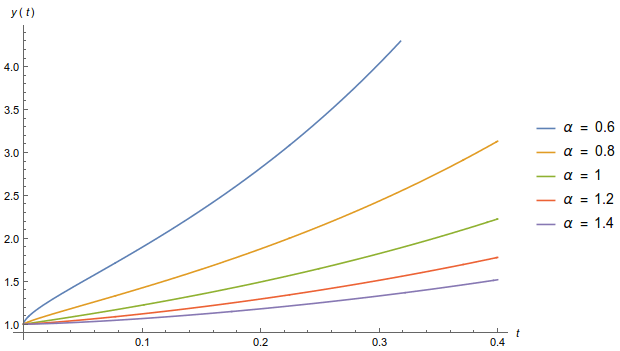
\includegraphics[scale=0.7]{images/Mittag-Leffler-Solution}
    \caption{Various solution curves for \eqref{eq:fde-1} with $ \beta = 1 $ and the initial conditions specified in \eqref{eq:fde-1-ic}}.
\end{figure}

\subsection{Solution to a multi-order initial value problem via Laplace transforms}
%\addcontentsline{toc}{section}{Solution to a Multi-Order Fractional Differential Equation}
The Laplace transform technique can be applied to multi-order fractional differential equations as well. The following proposition demonstrates how.
\begin{mdframed}[innertopmargin=10pt]
\begin{lemma}
	The initial value problem,
	\begin{align}
	    \label{eq:fde-multi-order}
	    \prescript{}{0}{\mathcal{D}}^{\Lambda}y(t) + \prescript{}{0}{\mathcal{D}}^{\lambda}y(t) = f(t)
	\end{align}
	has solution, given by
	\begin{align*}
		y(t) = C g(t) + \int_0^t g(t-\tau)f(\tau) d\tau
	\end{align*}
where
	\begin{align*}
		C &= \prescript{}{0}{\mathcal{D}}^{\Lambda-1}y(0) + \prescript{}{0}{\mathcal{D}}^{\lambda-1}y(0) \\
		g(t) &= t^{\Lambda - 1} E_{\Lambda - \lambda, \Lambda}(-t^{\Lambda - \lambda}).
	\end{align*}
\end{lemma}
\end{mdframed}
This proof follows the technique outlined in \cite{Podlubny1999}.
\begin{proof}

	Taking the Laplace transform of both sides of \ref{eq:fde-multi-order} and using the result of lemma \ref{lem:lap_rld}
	we get that 
	\begin{align*}
		\laplace{\prescript{}{0}{\mathcal{D}}^{\Lambda}y(t)} + \laplace{\prescript{}{0}{\mathcal{D}}^{\Lambda}y(t)} &= \laplace{f(t)} \\
		s^\Lambda Y(s) + s^\lambda Y(s) - \prescript{}{0}{\mathcal{D}}^{\Lambda-1}y(0) - \prescript{}{0}{\mathcal{D}}^{\lambda-1}y(0) &= F(s).
	\end{align*}
	Note that 
	\begin{align*}
	    C &= \prescript{}{0}{\mathcal{D}}^{\Lambda-1}y(0) + \prescript{}{0}{\mathcal{D}}^{\lambda-1}y(0) 
	\end{align*}
	 
	is a constant so we write
	\begin{align*}
		Y(s) &= \frac{C + F(s)}{s^\Lambda + s^\lambda} \\
			&= \left( C + F(s)\right) \frac{s^{-\lambda}}{s^{\Lambda-\lambda} + 1}.
	\end{align*}
	
	Let 
	\begin{align*} 
	    G(s) = \frac{s^{-\lambda}}{s^{\Lambda-\lambda} + 1} 
	\end{align*}
	and by using lemma \ref{lem:lap_mit_2} with $ \alpha = \Lambda - \lambda $ and $ \gamma = \Lambda $
	we get that 
	\begin{align*}
	    g(t) = t^{\Lambda  -1}E_{\Lambda - \lambda, \Lambda}(-t^{\Lambda - \lambda})
	\end{align*} where $ \laplace{g(t)} = G(s) $.
	
	Then using the Laplace convolution theorem we get that 
	\begin{align*}
		y(t) = C g(t) + \int_0^t g(t-\tau)f(\tau) d\tau
	\end{align*}
	where
	\begin{align*}
		C &= \prescript{}{0}{\mathcal{D}}^{\Lambda-1}y(0) + \prescript{}{0}{\mathcal{D}}^{\lambda-1}y(0)  \\
		g(t) &= t^{\Lambda - 1} E_{\Lambda - \lambda, \Lambda}(-t^{\Lambda - \lambda}).
	\end{align*}
\end{proof}

\begin{figure}[H]
    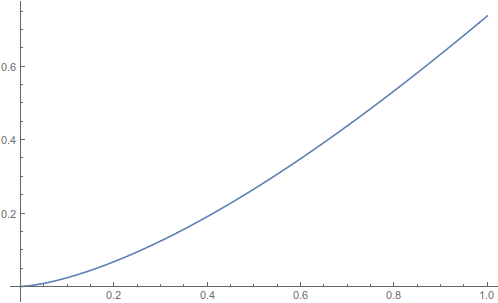
\includegraphics[scale=0.7]{images/Mittag-Leffler-Solution-2}
    \caption{A solution curve for \eqref{eq:fde-multi-order}, with $ C = 1, \Lambda = \frac{3}{2}, \lambda = \frac{1}{2} $ and $ f(t) = \cos(t) $. }.
\end{figure}

Also note that this differential equation is in terms of Riemann-Liouville derivatives. If we were to specify
initial conditions we would be compelled to specify them in terms of fractional derivatives, so we leave them
unspecified here to see the solution in general.




\subsection{Other techniques for ordinary fractional differential equations}

As hinted at previously we could just use the results of lemma \ref{lem:rld_mittag} to potentially \emph{guess and check} a solution to \ref{eq:fde-multi-order}. This is certainly the case and especially when combined with the result of \ref{lem:rld_power} this becomes quite possible. However direct application of fractional derivatives or integrals to functions is \emph{tricky}. The techniques often hinge off changes of variables in integrals, such as in the proofs of many of the results in section \ref{sec:operators} which are sometimes non-obvious. That's why we have presented these solutions via the Laplace transform methods. These results using these methods are \emph{almost trivial}. In fact fractional differential equations are often solved by \emph{dual tranform} techniques. That is by using something like a Laplace or Fourier transform. (In the next subsection we will use the Fourier transform.)

There are other methods for solving fractiona differential equations. These include a technique using Mellin trasnforms \cite{Podlubny1999, Kober1940, Samko1993, Butera2014}, orthogonal polynomials \cite{Podlubny1999}, power series \cite{Podlubny1999, Samko1993, Arikoglu2007} and a particularly interesting method called Babenko Symbolic Calculus \cite{Podlubny1999, Gorenflo1997b}.

\subsection{Solutions to partial fractional differential equations}
Its not just ordinary fractional differential equations that can be solved by analytic techniques. Some partial fractional differential equations admit an analytic solution and that is what we will look at in this subsection.

\begin{mdframed}[innertopmargin=10pt]
\begin{proposition}
    \label{prop:nig_frac}
    The following time fractional partial differential equation \footnote{Here $ \prescript{}{0}{\mathcal{D}}^\alpha_t $ refers to the Riemann-Liouville fractional derivative with respect to $ t $.}
    \begin{align}
        \label{eq:nig_frac}
        \prescript{}{0}{\mathcal{D}}^\alpha_t u(x,t) = \lambda^2 \frac{\partial^2}{\partial x^2}u(x,t)
    \end{align}
    with $ 0 < \alpha < 1 $ along with the intial condition
    \begin{align*}
        \prescript{}{0}{\mathcal{D}}^{\alpha-1}_t u(x,t) \Big|_{t=0} = \psi(x)
    \end{align*}
    has the solution
    \begin{align*}
        u(x,t) = \int_{-\infty}^\infty \xi(x - \eta, t) \psi(\eta) d\eta
    \end{align*}
    where
    \begin{align*}
        \xi(x,t) = \frac{1}{\pi} \int_0^\infty t^{\alpha - 1} E_{\alpha, \alpha}(-\lambda^2\omega^2t^\alpha)\cos(\omega x)d\omega.
    \end{align*}
\end{proposition}
\end{mdframed}
\begin{proof}
    Taking the Fourier transform of both sides of \eqref{eq:nig_frac} yeilds
    \begin{align*}
        \prescript{}{0}{\mathcal{D}}^\alpha_t \hat{u}(\omega,t) = -\omega^2\lambda^2 \hat{u}(\omega, t)
    \end{align*}
    where $ \hat{u}(\omega, t) = \mathcal{F}_x\left\{ u(x,t) \right\} $. \footnote{Here $ \mathcal{F}_x $ refers to the Fourier transform with respect to $ x $}
    Rearranging and taking the Laplace transform with the help of lemma \ref{lem:lap_rld} gives us
    \begin{align*}
        s^\alpha\hat{U}(\omega, s) + \lambda^2\omega^2 \hat{U}(\omega,s) = \hat{\psi}(\omega)
    \end{align*}
    where $ \hat{U}(\omega, s) $ is the Fourier and Laplace transform of $ u(x,t) $ with respect to $ x $ and $ t $ respectively.
    So we have that
    \begin{align*}
        \hat{U}(\omega, s) = \frac{\hat{\psi}(\omega)}{s^\alpha + \lambda^2\beta^2}.
    \end{align*}
    By appealing to lemma \ref{lem:lap_mit_2} we can invert the Laplace transform to get
    \begin{align*}
        \hat{u}(\omega, t) = \psi(\omega)t^{\alpha-1} E_{\alpha, \alpha}(-\lambda^2\beta^2t^\alpha).
    \end{align*}
    Now this is clearly the product of Fourier transforms so the inverse transform is given by the convolution of two functions, and so
    \begin{align*}
        u(x,t) = \int_{-\infty}^\infty \xi(x - \eta, t) \psi(\eta) d\eta
    \end{align*}
    where
    \begin{align*}
        \xi(x,t) = \frac{1}{2\pi} \int_{-\infty}^\infty t^{\alpha - 1} E_{\alpha, \alpha}(-\lambda^2\omega^2t^\alpha)e^{i\omega x}d\omega.
    \end{align*}
    but by acknowledging that $ E_{\alpha, \alpha}(-\lambda^2\omega^2t^\alpha)e^{i\omega x} $ is even in $ \omega $ this can be written as 
    \begin{align*}
        \xi(x,t) = \frac{1}{\pi} \int_0^\infty t^{\alpha - 1} E_{\alpha, \alpha}(-\lambda^2\omega^2t^\alpha)\cos(\omega x)d\omega.
    \end{align*}
\end{proof}
    Podlubny \cite{Podlubny1999} takes this result further and shows that when coupled with the limiting condition
    \begin{align*}
        \lim_{x \lra \pm \infty} u(x,t) = 0
    \end{align*}
    we have
    \begin{align*}
        \xi(x,t) = \frac{1}{2\lambda} t^{\rho-1}W_{-\rho,\rho}\left(-\frac{|x|}{\lambda t^\rho}\right)
    \end{align*}
    but showing this result requires a number of techniques not otherwise explored in this thesis.
    
    Note that this fractional partial differential equation is essentially a time fractional heat equation. It's actually known as the Nigmatullin fractional diffusion equation \cite{Podlubny1999, Nigmatullin1986}. Interestingly Nigmatullin has published many papers on physical notions and examples of fractional differential equations and this particular version of the diffusion equation can be seen as having physical significance \cite{Nigmatullin1986, Nigmatullin1992, Meerschaert2011}. 
    
It should be noted that by replacing the Riemann-Liouville fractional derivative with a Caputo fractional derivative we get a similar result \cite{Nikolova2010}. We'll formalize this assertion with the following proposition.

\begin{mdframed}[innertopmargin=10pt]
\begin{proposition}
	\label{prop:frac_diff_2}
    The following time fractional partial differential equation
    \begin{align}
        \label{eq:nig_frac_2}
        \prescript{C}{0}{\mathcal{D}}^\alpha_t u(x,t) = \lambda^2 \frac{\partial^2}{\partial x^2}u(x,t)
    \end{align}
    with $ 0 < \alpha < 1 $
    along with the initial condition
    \begin{align*}
        u(x,t)|_{t=0} = \psi(x)
    \end{align*}
    has a solution given by
    \begin{align*}
        u(x,t) = \int_{-\infty}^\infty \xi(x - \eta, t)\psi(\eta)d\eta
    \end{align*}
    where
    \begin{align*}
        \xi(x,t) = \frac{1}{2\pi} \int_{-\infty}^\infty e^{-i\omega x}E_{\alpha, 1}(-\lambda^2 \omega^2 t^\alpha) d\omega.
    \end{align*}
\end{proposition}
\end{mdframed}
This proof follows in much the same way as for proposition \ref{prop:nig_frac} but with lemma \ref{lem:cap_laplace} instead of lemma \ref{lem:lap_rld}. We also use the same notation as in the previous solution.
\begin{proof}
Taking the Fourier and Laplace transforms of \eqref{eq:nig_frac_2} with the help of lemma \ref{lem:cap_laplace} results in
\begin{align*}
    s^{\alpha}\hat{U}(\omega, s) - s^{\alpha-1}\hat{\psi}(\omega) = -\lambda^2\omega^2\hat{U}(\omega, s)
\end{align*}
and thus
\begin{align*}
    \hat{U}(\omega,s) = \frac{s^{\alpha-1}\hat{\psi}(\omega)}{(s^\alpha + \lambda^2\omega^2)}.
\end{align*}
Again, inverting the Laplace transform with the help of \ref{lem:lap_mit_2} we get that
\begin{align*}
    \hat{u}(\omega,t) = E_{\alpha,1}(-\omega^2\lambda^2t^\alpha) \hat{\psi}(\omega)
\end{align*}
and now by following exactly the same steps as for proposition \ref{prop:nig_frac} the result follows. 
\end{proof}
Due to the fact that this fractional partial differential equation is specified with an integer order initial condition it is in some sense more usefull from a physical modelling perspective. 

\subsubsection{A note on Fourier Transform techniques for space fractional diffusion}
It might look like a good idea to use the results in lemmas \ref{lem:rld_fourier} and \ref{lem:cap_fourier} to try and attack a \emph{space fractional} diffusion problem. Unfortunately it is not as simple as that. The reason comes down to the fact that $ (i\omega)^\alpha $ hasn't been defined for non-integer $ \alpha $ and negative $ \omega $. If you use the definition $  (i\omega)^\alpha = |\omega|^\alpha\left(cos\left(\frac{\alpha\pi}{2}\right) + i\operatorname{sgn}(\omega)\sin\left(\frac{\alpha\pi}{2}\right)\right) $ then one can use this along with the Riesz fractional derivative to tackle space fractional diffusion. The definition of the Riesz fractional derivative of a function is
\begin{align}
	\prescript{R}{}{D}^\alpha f(x) = \mathcal{F} \{ -|\omega|^\alpha \hat{f}(\omega) \}
\end{align}
and this definition along with principle value definition of $ (i\omega)^\alpha $ given above give a way of dealing with space fractional diffusion.

Although we won't really investigate this field in this thesis fractional diffusion has a very rapidly growing and important field with applications in mathematical biology, finance and physics \cite{Henry2010}.
ma
\clearpage
